\begin{figure}
\centering\fontsize{9}{9}\fontfamily\sfdefault\selectfont
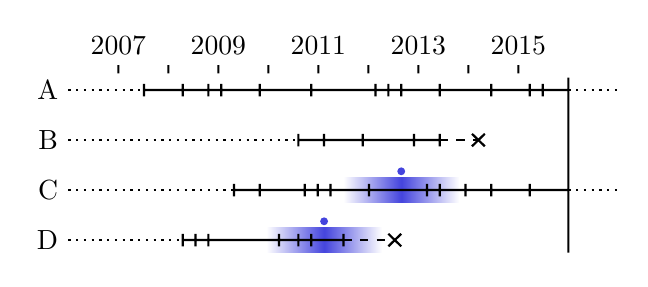
\begin{tikzpicture}[x=0.25in, y=0.125in,thick]

% Text first, since it defines a bunch of coordinates and doesn't
% overlap anything.
\foreach \x/\xtext in {2/2007, 4/2009, 6/2011, 8/2013, 10/2015}
  \node[above] (\xtext) at (\x,8) {\xtext} ;

\foreach \y/\ytext in {7/A, 5/B, 3/C, 1/D} {
  \node[left] (\ytext) at (1,\y) {\ytext} ;
  \coordinate (u\ytext) at ([yshift=0.03125in]\ytext);
  \coordinate (d\ytext) at ([yshift=-0.03125in]\ytext);
}

% The shaded areas must be drawn next, since they are underneath
% stuff.  For some damn reason, you can't put two circles or
% rectangles in one \path construct.
\definecolor{c44d}{RGB}{68,68,221}
\begin{scope}[fill=c44d]
  \fill (6.1144,1.7502) circle (0.05cm);
  \fill (7.6573,3.7502) circle (0.05cm);
\end{scope}

\begin{scope}[shading=axis,
              left color=white, right color=white, middle color=c44d]
  \shade (4.9573,1.4996) rectangle (7.2717,0.4996);
  \shade (6.5002,3.4996) rectangle (8.8146,2.4996);
\end{scope}

% Now, all of the tick marks. All of them.
\draw
  % "contemporary capture" line
  (11,7.5) coordinate (cline) -- (11,0.5)
  % year ticks
  \foreach \x in {2,...,10} {(\x,8) -- +(0,-0.3333333)}

  % A line
  \foreach \x in {
     2.5141, 3.2855, 3.7998, 4.0570, 4.8284, 5.8570, 7.1428, 7.3999,
     7.6571, 8.4285, 9.4571,10.2286,10.4857
  }
  { (\x,0 |- uA) -- (\x,0 |- dA) }

  % B line
  \foreach \x in {
    5.5999, 6.1142, 6.8856, 7.9142, 8.4285
  }
  { (\x,0 |- uB) -- (\x,0 |- dB) }

  (9.0717,0 |- uB) -- (9.3289,0 |- dB)
  (9.0717,0 |- dB) -- (9.3289,0 |- uB)

  % C line
  \foreach \x in {
     4.3143, 4.8286, 5.7287, 5.9858, 6.2430, 7.0144, 8.1716, 8.4287,
     8.9430, 9.4573,10.2288
  }
  { (\x,0 |- uC) -- (\x,0 |- dC) }

  % D line
  \foreach \x in {
     3.2860, 3.5431, 3.8003, 5.2146, 5.6003, 5.8575, 6.5004
  }
  { (\x,0 |- uD) -- (\x,0 |- dD) }

  (7.3999,0 |- uD) -- (7.6571,0 |- dD)
  (7.3999,0 |- dD) -- (7.6571,0 |- uD)

% The horizontal lines are drawn after everything else
% to minimize the number of times the dash pattern has to be changed.
  (A -| 2.5141,0) -- (A -| cline)
  (B -| 5.6000,0) -- (B -| 8.4285,0)
  (C -| 4.3143,0) -- (C -| cline)
  (D -| 3.2857,0) -- (D -| 6.5000,0)
;

\draw [dotted]
  (A) -- (A -| 2.5141,0)  (A -| cline) -- +(1,0)
  (B) -- (B -| 5.6000,0)
  (C) -- (C -| 4.3143,0)  (C -| cline) -- +(1,0)
  (D) -- (D -| 3.2857,0)
;

\draw [dashed]
  (B -| 8.4285,0) -- (B -| 9.2000,0)
  (D -| 6.5000,0) -- (D -| 7.5288,0)
;
\end{tikzpicture}
\caption{The life cycles of four hypothetical websites. Tick marks are
  Wayback Machine snapshots; the vertical bar is our contemporary data
  capture; blue shaded areas indicate possible censorship events.}
\label{f:survival-diagram}
\end{figure}
\endinput
